\vspace{-2mm}
\section{Gated Linear Attention}
\vspace{-2mm}
\label{sec:gla}




The linear recurrence in Eq.~\ref{eq:simple_linear_attention} does not have a decay term or a forget gate, which has been shown to be crucial in RNNs~\citep{HochSchm97,cho2014learning,unreasonable-forget-gate}. The lack of a decay term makes it difficult for a model to ``forget'' information, and has been hypothesized to be partially responsible for the instability of linear attention in long-context tasks~\citep{buckman2024}. Recent works~\citep{sun2023retentive,qin2023scaling} obtain better performance through incorporating a global, \emph{non-data-dependent}  decay factor\footnote{This can be viewed as linear attention with  ALiBi position encodings \cite{alibi2021}.
In practice these works also incorporate  rotary position embeddings \citep[RoPE;][]{rope}.}
$\gamma \in (0, 1)$ into linear attention:
$ \rmS_t = \gamma \rmS_{t-1} + \vk_t^\intercal \vv_t$.
The use of a single $\gamma$ is designed to preserve the attention-style parallel form for efficient training. 
In this work, we consider a data-dependent gating mechanism for linear attention. We show that despite having a more expressive gating factor, the resulting gated linear attention (GLA) layer still admits a hardware-efficient chunkwise form for efficient training.


\vspace{-2mm}
\subsection{Recurrent and Parallel Form of GLA}
\vspace{-2mm}
\label{ssec:gla}
\begin{table*}[t!]
%
\footnotesize
\centering
\scalebox{0.8}{
\begin{tabular}{l l l }
\toprule
   Model  &  Parameterization  & Learnable parameters   \\
   \midrule
 %
    %
    Mamba \cite{Gu2023MambaLS} & $\rmG_t = \exp(-( \mathbf{1}^{\intercal}\balpha_t)\odot \exp(\mA)),\quad \balpha_t =\operatorname{softplus}(\vx_t\mW_{\alpha_1}\mW_{\alpha_2})$ & $\mA \in \mathbb{R}^{d_k \times d_v}, \quad \mW_{\alpha_1} \in \mathbb{R}^{d \times \frac{d}{16}}, \quad \mW_{\alpha_2} \in  \mathbb{R}^{\frac{d}{16} \times d_v}$ \\
    Mamba-2 \cite{mamba2} & $\rmG_t = \gamma_t \mathbf{1}^\intercal\mathbf{1}, \quad \gamma_t = \exp\left(-\operatorname{softplus}\left(\vx_t \mW_{\gamma}\right)\exp\left(a\right)\right)$  &  $\mW_{\gamma}
    \in \mathbb{R}^{d \times 1}, \quad a\in \mathbb{R}$ \\
    mLSTM \cite{beck2024xlstm, peng2021random} &  $\rmG_t = \gamma_t \mathbf{1}^\intercal\mathbf{1}, \quad \gamma_t = \sigma\left(\vx_t \mW_{\gamma}\right)$ &  $\mW_{\gamma} \in \mathbb{R}^{d \times 1}$ \\
    Gated Retention \cite{Sun2024YouOC} &
  $\rmG_t = \gamma_t \mathbf{1}^\intercal\mathbf{1}, \quad \gamma_t = \sigma\left(\vx_t \mW_{\gamma}\right)^{\frac{1}{\tau}}$ &  $\mW_{\gamma} \in \mathbb{R}^{d \times 1}$ \\
        DFW \cite{mao-2022-fine,recurrent_linear_xfmr}
        %
        & $\rmG_t = \balpha_t^\intercal \bbeta_t, \quad \balpha_t = \sigma(\vx_t \mW_{\alpha}), \quad \bbeta_t = \sigma(\vx_t \mW_{\beta})$ & $ \mW_{\alpha} \in \mathbb{R}^{d \times d_k}, \quad \mW_{\beta} \in \mathbb{R}^{d \times d_v}$   \\
    GateLoop \cite{gatedloop} & $\rmG_t = \balpha_t^\intercal \mathbf{1}, \quad \balpha_t = \sigma\left(\vx_t\mW_{\alpha_1}\right) \exp\left( \vx_t\mW_{\alpha_2} \mathbf{i} \right) $ & $\mW_{\alpha_1} \in \mathbb{R}^{d\times d_k}, \quad \mW_{\alpha_2}\in \mathbb{R}^{d \times d_k}$ \\
        %
  HGRN-2 \cite{qin2024hgrn2} &  $\rmG_t = \balpha_t^\intercal\mathbf{1}, \quad \balpha_t = \boldsymbol{\gamma} + (1-\boldsymbol{\gamma} ) \sigma(\vx_t \mW_{\alpha})$   & $\mW_{\alpha} \in \mathbb{R}^{d \times d_k}, \quad \boldsymbol{\gamma}  \in (0, 1)^{d_k}$
  \\
  RWKV-6 \cite{peng2024eagle} & $\rmG_t =\balpha_t^\intercal\mathbf{1}, \quad \balpha_t = \exp\left(-\exp\left(\vx_t\mW_{\alpha}\right)\right)$ & $\mW_{\alpha} \in \mathbb{R}^{d \times d_k} $ \\
  Gated Linear Attention (GLA) & $\rmG_t = \balpha_t^\intercal \mathbf{1}, \quad \balpha_t = \sigma\left(\vx_t\mW_{\alpha_1}\mW_{\alpha_2}\right)^{\frac{1}{\tau}}$ & $\mW_{\alpha_1} \in \mathbb{R}^{d\times 16}, \quad \mW_{\alpha_2}\in \mathbb{R}^{16 \times d_k}$ \\
  \bottomrule
\end{tabular}
}
\vspace{1mm}
%
\vspace{-4mm}
\caption{Gated linear attention formulation of recent  models, which vary in their parameterization of $\rmG_t$. The bias terms are omitted.}
\vspace{-4mm}
\label{tab:G_param}
\end{table*}

\paragraph{Recurrent form.} GLA has a 2D forget gate \(\rmG_t \in (0,1)^{d_k \times d_v}\) that varies over time:
\[
\rmS_t = \rmG_t \odot \rmS_{t-1} + \vk_t^{\top} \vv_t,
\]
where we now allow the hidden state to have varying dimensions.
This Hadamard product-based  recurrent form is very general and encompasses many recent RNNs with 2D hidden states, as listed in Table~\ref{tab:G_param}. 

Central to the design of gated linear attention  is the parameterization of \(\rmG_t\) which requires a balance between \textit{parameter-efficiency}, \textit{state size}, 
%
and \textit{training efficiency}.
A na\"{i}ve mapping $\vx_t \mapsto \rmG_{t}$ to obtain a data-dependent gating matrix would require a matrix of size $d \cdot d_k \cdot d_v$, which would be parameter-inefficient. \citet{mao-2022-fine} propose a more efficient outer-product-based low-rank parameterization (\(\rmG_t = \balpha_t^{\top} \bbeta_t\)), which requires $d \cdot d_v + d  \cdot d_k$ parameters.\footnote{However, \citet{mao-2022-fine} works with only the recurrent form and materializes the hidden states for all time steps in HBM. In Appendix \ref{sec:ggla} we give a new algorithm that reformulates the model in a matrix-multiply-based parallel form, which can make use of (an extension of) \textsc{FlashLinearAttention} for efficient training.}

%
%
%

In Mamba~\cite{Gu2023MambaLS}, \(\rmG_t\) is obtained by combining a  \emph{data-independent} learnable matrix \(\mA\) with a data-dependent vector $\balpha_t$, which allows the matrix to be full rank. However, this prevents the use of tensor cores because it cannot be reformulated into a matrix-multiply format, as discussed in  \citet{mamba2}. The lack of a compact matrix-multiply form  necessitates the materialization of each time step's hidden states. To reduce high I/O costs, \citet{Gu2023MambaLS} develop a hardware-aware algorithm that materializes the hidden states {exclusively} in  SRAM rather than in HBM. Due to limited SRAM capacity, this approach cannot scale to larger hidden states, which, as we will show in our experiments, results in suboptimal performance on recall-intensive tasks. Mamba-2 \cite{mamba2} addresses this limitation with a more {restricted} gating mechanism: \(\rmG_t = \gamma_t \mathbf{1}^T \mathbf{1}\), where \(\gamma_t \in (0,1)\) is a scalar, which makes it possible to to reformulate the recurrence in matrix-multiply form, enabling the use of tensor cores and larger  state sizes. This \emph{scalar} data-dependent gating is also used in \citet{peng2021random}, \citet{Sun2024YouOC}, and \citet{beck2024xlstm}. 

%

%
%
%
%
%
%
%
 
%

 %

 
 This paper adopts a middle ground between the scalar and the fully low-rank parameterization by using $\rmG_{t} = \balpha_t ^\top \mathbf{1}$.\footnote{Our preliminary experiments with the $\rmG_t = \balpha_t^\top \bbeta_t$ parameterization resulted in only marginal improvements over $\rmG_{t} = \balpha_t ^\top \mathbf{1}$.}
 %
 %
This results in the following recurrent form,
%
\begin{align}
\rmS_t =  (\balpha_t^{\top} \mathbf{1}) \odot \rmS_{t-1} + \vk_t^{\top} \vv_t = \text{Diag}(\balpha_t)  \rmS_{t-1} + \vk_t^{\top} \vv_t, 
\label{eq:gla-simple}
\end{align}
%
where $\balpha_t$ is parameterized via a low-rank linear layer followed by sigmoid on $\vx_t$ (see \S\ref{sec:gla-full}). Note that the above formulation 
 is general and  encompasses several recent RNNs \cite{gatedloop, qin2024hgrn2, peng2024eagle}. Thus, the hardware-efficient GLA implementation (described next) could be directly used or adapted to other models. 

%

%





\vspace{-2mm}
\paragraph{Parallel form.} 
We now describe a parallel form GLA for parallelizing across sequence length. Unrolling Eq.~\ref{eq:gla-simple} gives
\begin{equation*}
\rmS_t = \sum_{i=1}^{t} \left(\left(\prod_{j=i+1}^{t}\balpha_{j}^{\top}\mathbf{1}\right) \odot \vk_i^{\top} \vv_i \right)    
\label{eq:gla_parallel}
\end{equation*}
Letting $\vb_t := \prod_{j=1}^{t} \balpha_j$, we can rewrite the above as 
\begin{align*}
\vo_t = \vq_t \rmS_t &= \vq_t \sum_{i=1}^{t} \left( \left(\frac{\vb_t}{\vb_i} \right)^{\top} \mathbf{1} \right) \odot \vk_i^{\top} \vv_i \\ &= \sum_{i=1}^{t}(\vq_t \odot \vb_t) \left(\frac{\vk_i}{\vb_i}\right)^{\top} \vv_i
\end{align*}
where the division is element-wise. Letting $\rmB \in (0,1)^{L \times d}$ be the matrix obtained from stacking $\vb_t$'s,  the parallel form is:
\begin{equation*}
\rmO = \left(\left(\underbrace{(\rmQ \odot \rmB) \left(\frac{\rmK}{\rmB}\right)^{\top}}_{\mathbf{P}} \right) \odot \rmM \right) \rmV.
\label{eq:parallel_gla}
\end{equation*}
However, this form is not numerical stable as $\vb_t$  is the cumulative product of gate values in $\balpha_j \in (0, 1)^{1 \times d}$, and thus can be extremely small when $t$ is large, making $ \frac{\mathbf{K}}{\rmB}$ explode. To handle this, we can compute in log space for $\mathbf{P}$,\footnote{This form resembles extrapolatable position encoding~\citep{xpos} in that the term inside the exponential can be viewed as a  \textit{data-dependent} relative position factor. }
\begin{align}
    \vspace{-6mm}
    \mathbf{P}_{ij} = \sum_{k=1}^{d} \mathbf{Q}_{ik} \mathbf{K}_{jk} \, \exp(\log \rmB_{ik}-\log\rmB_{jk}), \quad i \ge j,
    \label{eq:log-semiring}
    \vspace{-6mm}
\end{align}
where $k$ denotes feature indices. 
However, unlike vanilla linear attention, as Eq. \ref{eq:log-semiring} cannot be represented via a standard matmul, and it cannot make use of half-precision matmuls on tensor cores. We will show in \S\ref{subsec:flash-gla} how a secondary-level chunking mechanism can enable the use of half-precision matmuls for most computations while maintaining numerical stability, as illustrated in Figure~\ref{fig:gla_tiling}.


\def\width{16}
\def\hauteur{16}
%
%
%

\definecolor{orange}{RGB}{250,230,200}
\definecolor{gray}{RGB}{220,220,220}
\definecolor{pink}{RGB}{247,206,205}

\begin{figure}[t]
\vspace{-2mm}
    \centering
        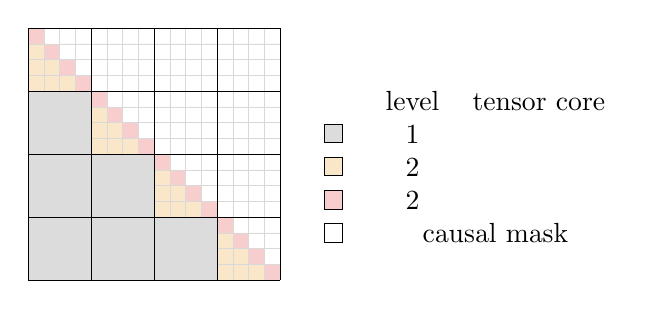
\begin{tikzpicture}[x=0.2cm, y=0.2cm]
    %
    %
    
    %
    %
    %

    \foreach \y in {0, ..., 15}{
        \foreach \x in {0, ...,  15} {%
        %
            \pgfmathsetmacro{\col}{ifthenelse(\x<15-\y,"orange",ifthenelse(\x==\y+1,"white","white"))}
       \fill[\col] (\x,\y) rectangle (\x+1,\y+1);
       }
    }
    \foreach \y in {0, ..., 15}{
       \fill[pink] (\y,15-\y) rectangle (\y+1,15-\y+1);
       }
    
   
    \draw[step=0.20cm, line width=0.05mm, black!15!white, fill=orange] (0,0) grid (\width,\hauteur);
    \foreach \x in {0, ..., 8} {%
    %
    \fill[gray] (\x,0) rectangle (\x+4,4);
    }
        \foreach \x in {0, ..., 4} {%
    %
    \fill[gray] (\x,4) rectangle (\x+4,8);
    }
    \foreach \x in {0, ..., 1} {%
    %
    \fill[gray] (\x,8) rectangle (\x+3,12);
    }
    
    \foreach \x in {0, ..., 1} {%
    %
    \fill[gray] (\x,8) rectangle (\x+3,12);
    }


    \draw[step=0.8cm, line width=0.1mm, black!10!black, fill=orange] (0,0) grid (\width,\hauteur);

    %
    %
    %
      
    %
    %
    %
    %
        \node 
        [shape=rectangle,fill=white, 
        align=center](table2) at (28.0,7.0) {

            \begin{tabular}{lcc} \toprule
                 & level & tensor core   \\ 
            \begin{tikz}
                \node [draw,fill=gray] {};
            \end{tikz} & 1 & $\checkmark$\\
                \begin{tikz}
                \node [draw,fill=orange] {}; 
            \end{tikz} & 2 & $\checkmark$\\
             \begin{tikz}
                \node [draw,fill=pink] {}; 
            \end{tikz} & 2 & $\text{\xmark}$\\
                 \begin{tikz}
                \node [draw,fill=white] {}; 
            \end{tikz} & \multicolumn{2}{ c}{causal mask}\\
                 %
                \bottomrule
            \end{tabular}
        };

%
    \end{tikzpicture}
\vspace{-2mm}
    \caption{
    Attention-style map to illustrate the chunkwise computations in GLA. The inter-chunk dependencies (in gray) 
    are not directly computed in the chunkwise form (only computed in the parallel form).
    The intra-chunk dependencies are modeled via secondary chunking/tiling where the inter-sub-chunk part (in orange) is computed by half-precision matmuls while the intra-sub-chunk part (in pink) is computed in full precision in log space. 
    }
    \label{fig:gla_tiling}

\end{figure}





\vspace{-2mm}
\subsection{Chunkwise Parallel Form of GLA}
\vspace{-2mm}
We derive a chunkwise form of GLA similar to the chunkwise form of basic linear attention (\S\ref{background:lin-chunkwise}). Here the intra-chunk operation implements the above parallel form at the chunk-level to obtain $\rmO^{\text{intra}}$. For inter-chunk, we have
\begin{align*}
\mathbf{\Lambda}_{iC+j} &= \frac{\vb_{iC+j}}{\vb_{iC}},  \mathbf{\Gamma}_{iC+j} = \frac{\vb_{(i+1)C}}{\vb_{iC+j}}, 
\bgamma_{i+1} = \frac{\vb_{(i+1)C}}{\vb_{iC}},  
 \\
\rmS_{[i+1]} &= \left(\bgamma_{i+1}^{\top}\mathbf{1}\right)  \odot \rmS_{[i]} + \left(\rmK_{[i+1]} \odot \mathbf \Gamma_{[i+1]} \right)^{\top}
\rmV_{[i+1]},  \\
\rmO^{\text{inter}}_{[i+1]} &= \left(\rmQ_{[i+1]} \odot \mathbf \Lambda_{[i+1]}\right) \rmS_{[i]}. 
\end{align*}
Intuitively, $\mathbf \Lambda_{[i+1]} $ encodes the cumulative decay from the start of a chunk which will be used to propagate the hidden states from the previous chunk $\rmS_{[i]}$, while   $\mathbf \Gamma_{[i+1]}$ encodes the decay to the end of a chunk which will be used to accumulate information to be added to the next hidden state $\rmS_{[i+1]}$.
\vspace{-2mm}
\subsection{Hardware-Efficient GLA}
\vspace{-2mm}
\label{subsec:flash-gla}
With the chunkwise form in hand, we can adapt the \textsc{FlashLinear Attention} algorithm presented in \S\ref{sec:algorithm} to the gated case. The adaptation additionally relies on two crucial techniques described below. 
We give high-level intuitions in this section
and defer the full algorithms to Alg. \ref{algo:gla-chunk-scan-1-fwd}-\ref{algo:gla-chunk-scan-2-bwd} of Appendix~\ref{sec:gla_algo}.

\vspace{-2mm}

\paragraph{Secondary-level chunking.}
Unlike in ordinary linear attention, the intra-chunk computations in GLA {cannot} leverage half-precision matmuls (and thus tensor cores) due to log space computations (Eq.~\ref{eq:log-semiring}). To make better use of tensor cores, we use secondary-level chunking scheme, where a chunk is further divided into sub-chunks (i.e., another level of tiling) in the spirit of classic tiling techniques~\cite{flashattention1}. The  attention-like matrix $\rmP \in \R^{L\times L}$ is then computed in a chunkwise manner, as illustrated in Figure~\ref{fig:gla_tiling}. 
 Concretely, the interactions  between sub-chunks are computed via half-precision matmuls,\footnote{To reduce notational clutter, here we use the notations from the first-level chunking to express the key idea. The actual implementation is done with secondary-level chunks.}
\begin{align*}
 \rmP_{[i][j]} &=  \Big(\rmQ_{[i]} \odot \bLambda_{[i]} \Big) \Big(\rmK_{[j]} \odot \bGamma_{[j]} \odot  
 \frac{\vb_{iC}}{\vb_{(j+1)C}} \Big)^{\intercal} \in \mathbb{R}^{C\times C}.
 \label{eq:gla-subchunk-compute-p}
\end{align*}
This corresponds to the orange tiles in Figure~\ref{fig:gla_tiling}. For the intra-sub-chunk part (pink tiles in Figure~\ref{fig:gla_tiling}) we have to resort to Eq.~\ref{eq:log-semiring} and perform the matmul in full precision for stability.
With this two-level tiling strategy, the total amount of non-half-precision matmul FLOPs are greatly reduced, thus leading to wallclock improvements. We provide the Pytorch-style pseudo-code in Listing~\ref{a} of Appendix~\ref{sec:gla_algo}.

\vspace{-2mm}
\paragraph{Memory-efficient  \textnormal{$\dbalpha_t$} computation.} 
Past work \citep[\S 3.1]{mao-2022-fine} has claimed that GLA-like models have to materialize the matrix-valued hidden states of size $L \times d \times d$ in HBM to compute all the gradients $\dbalpha_t$, since $\dbalpha_t =  (\rmS_{t-1} \odot \mathbf d\rmS_{t}) \mathbf{1}$. 
%
We instead give the following \emph{closed form} formula for $\dblogalpha_t$, 
\begin{align*}
    \vdlogb_t &= \vq_t \odot \vdq_t - \vk_t \odot \vdk_t,  \hspace{4mm}
   \dblogalpha_t  = \sum_{t \leq i \leq L} \vdlogb_i,
\end{align*}
which can be easily obtained by taking the derivative with respect to 
 Eq.~\ref{eq:log-semiring} (see Appendix~\ref{sec:gla_algo} for full derivation). $\vdq_t$ and $\vdk_t$ can be  computed  as in Alg.~\ref{algo:la-chunk-bwd}.
 
\vspace{-2mm}
\subsection{GLA Transformer}
\vspace{-2mm}
\label{sec:gla-full}
We generalize the GLA layer to the multi-head case. Given $H$ heads, we have the following for each head $h \in [1, H]$,
\begin{align*}
    &\rmS^h_{t} =  \left( \left(\balpha_{t}^h\right)^{\top} \mathbf{1} \right)
    %
    \odot \rmS_{t-1}^h + \vk_t^{h \intercal} \, \vv^h_t   \in \mathbb{R}^{d'_k \times d'_v}, \\  %
& \vo^h_{t} = \vq_t^{h}\rmS_t^h    \in \mathbb{R}^{1 \times d'_v}, \\ &
\vo'_t = \operatorname{concat}(\lnorm(\vo^1_t), \dots, \lnorm(\vo^H_t)) \in \R^{1 \times d_v}, 
  \\
 &\vr_t = \operatorname{Swish}(\vx_t \mW_r + \vb_r)  \in \mathbb{R}^{1 \times d_v}, 
 \\ & \vy_t = (\vr_t \odot \vo'_t) \mW_{O}  \in \R^{1 \times d}. 
\end{align*}
Here we use separate key ($d_k$) and value ($d_v$) dimensions; $d'_k = d_k / H, d'_v = d_v / H$ are the per-head key/value dimensions. LayerNorm ($\lnorm$) is applied after the output of each head, while the output projection and output gating operate on the concatenation of head outputs \cite{sun2023retentive}. 

We then build up a Transformer-like model by interleaving multi-head GLA layers with feed-forward networks (FFN). Concretely, given layer $l$'s contextualized representation $\rmX^{(l)}$, we obtain  $\rmX^{(l+1)}$ via,
\begin{align*}
   %
   &\rmY^{(l)} = \operatorname{GLA}(\lnorm(\rmX^{(l)})) + \rmX^{(l)} \\ 
   & \rmX^{(l+1)} = \operatorname{SwiGLU}(\lnorm(\rmY^{(l)})) + \rmX^{(l)},
\end{align*}
where the $\swiglu$ FFN layer~\citep{touvron2023llama} is,
\begin{align*}
    \operatorname{SwiGLU}(\rmZ) = (\operatorname{Swish}(\rmZ \mW_1) \odot \rmZ \mW_2) \mW_{3}.
\end{align*}

\begin{table*}[t!]
\centering
\small
\addtolength{\tabcolsep}{-2.5pt}    
\begin{tabular}{l l|cc|cccccc|c}
\toprule
&   & \textbf{Wiki.}  &  \textbf{LMB.} &  \textbf{LMB.} & \textbf{PIQA} &    \textbf{Hella.} & \textbf{Wino.} & \textbf{ARC-e} &  \textbf{ARC-c} &  \textbf{Avg.}  \\
\textbf{Scale} & \textbf{Model}  & ppl $\downarrow$  &  ppl $\downarrow$  &  acc $\uparrow$  & acc $\uparrow$ &   acc\_norm $\uparrow$  & acc $\uparrow$  & acc $\uparrow$ & acc\_norm $\uparrow$ &  $\uparrow$ \\
\midrule
%
%
%
\textit{340M Params} &  Transformer++ & \text{28.39} & 42.69 & \text{31.0} & 63.3 & 34.0 &	50.4 & 44.5	& \text{24.2} &  41.2  \\
\textit{15B Tokens} &   RetNet  & 32.33 &	49.19 &	28.6 &	63.5 & 33.5 &	\text{52.5} &	44.5 &	23.4 &	 41.0 \\
&   Mamba  & \text{28.39} & \text{39.66} & 30.6 & \text{65.0} & \text{35.4} & 50.1 & \text{46.3} & 23.6 & \text{41.8} \\ 
%
&   GLA   & 28.65 &	43.35 &	30.3 &	64.8  & 34.5 & 51.4  & 45.1	 & 22.7 &	 41.5\\
%
%
\midrule 
%
 \textit{1.3B Params} &  Transformer++ & \text{16.85} & \text{13.44} &  \text{48.9} & 70.8 & 49.6 & 53.6 & 56.0 & 26.5 & 50.9 \\
\textit{100B Tokens}&   RetNet  & 18.64 & 17.27 & 43.3 & 70.0 & 47.3 & 52.5 & 54.8 & 25.6 & 48.9 \\
&  Mamba  & 17.06 & 13.89 & 46.2 & \text{72.2} &  40.1 & \text{54.1} &  \text{59.0} &	\text{28.2} & 50.0 \\
&  GLA  & 17.22 & 14.47 & 46.9 & 71.8 & \text{49.8} & 53.9 & 57.2 & 26.6 & \text{51.0}  \\
%
\bottomrule
\end{tabular}
\addtolength{\tabcolsep}{2.5pt}    
\centering
\vspace{-2mm}
\caption{GLA Transformer results against Transformer++ \citep{touvron2023llama}, RetNet \citep{sun2023retentive}, and Mamba \citep{Gu2023MambaLS}. All models are trained on the same subset of the SlimPajama dataset with the Mistral tokenizer. The 340M/1.3B models are trained for 15B/100B tokens respectively. The individual task performance is via zero-shot. We report the main results on the same set of tasks reported by \citet{Gu2023MambaLS}. See Appendix~\ref{app:d} for results on other benchmarks, including 5-shot results. The last column shows the average over all benchmarks that use (normalized) accuracy as the metric.}
\vspace{-3mm}
\label{tab:main_results}
\end{table*}

\vspace{-2mm}
\paragraph{Parameter allocation.}  As presented, our GLA layer employs two additional matrices  for predicting $\balpha_t, \vr_t$ (i.e., $\mW_\alpha, \mW_r$) compared to a regular softmax attention layer. %
%
For parameter-efficiency, we use a low-rank parameterization 
\begin{align*}
   \balpha_t = \sigma((\vx_t \mW^1_\alpha \mW^2_\alpha + \vb_\alpha)))^{\frac{1}{\tau}}   \in \R^{1 \times d_k},
\end{align*}
where $\mW^1_\alpha \in \R^{d \times 16}$, $\mW^2_\alpha \in \R^{16 \times d_k}$, and $\tau = 16$ is a temperature term to encourage model to have a slower forgetting rate. 
We further set $d_k = \frac{d}{2}$ and $d_v = d$ and use  full-rank parameterizations for ($\mW_Q, \mW_K, \mW_V, \mW_O, \mW_r$). 
%
Ultimately, one GLA layer collectively needs (roughly) $4d^2$ parameters, as in regular softmax attention. 

%
%
%
%
%
%
%
%
%